\subsection{Main Unit Power Supply}
\subsubsection{Block Diagram}
\createfigurewsvg{../Modular Design/Main-Unit-PSU/Figures/main-unit-psu.svg}{Main Unit Power Supply Architectural Diagram}{fig:main-unit-psu-bd}
\subsubsection{Schematic Diagram}
\begin{landscape}
  \begin{center}
  \begin{figure}[H]
    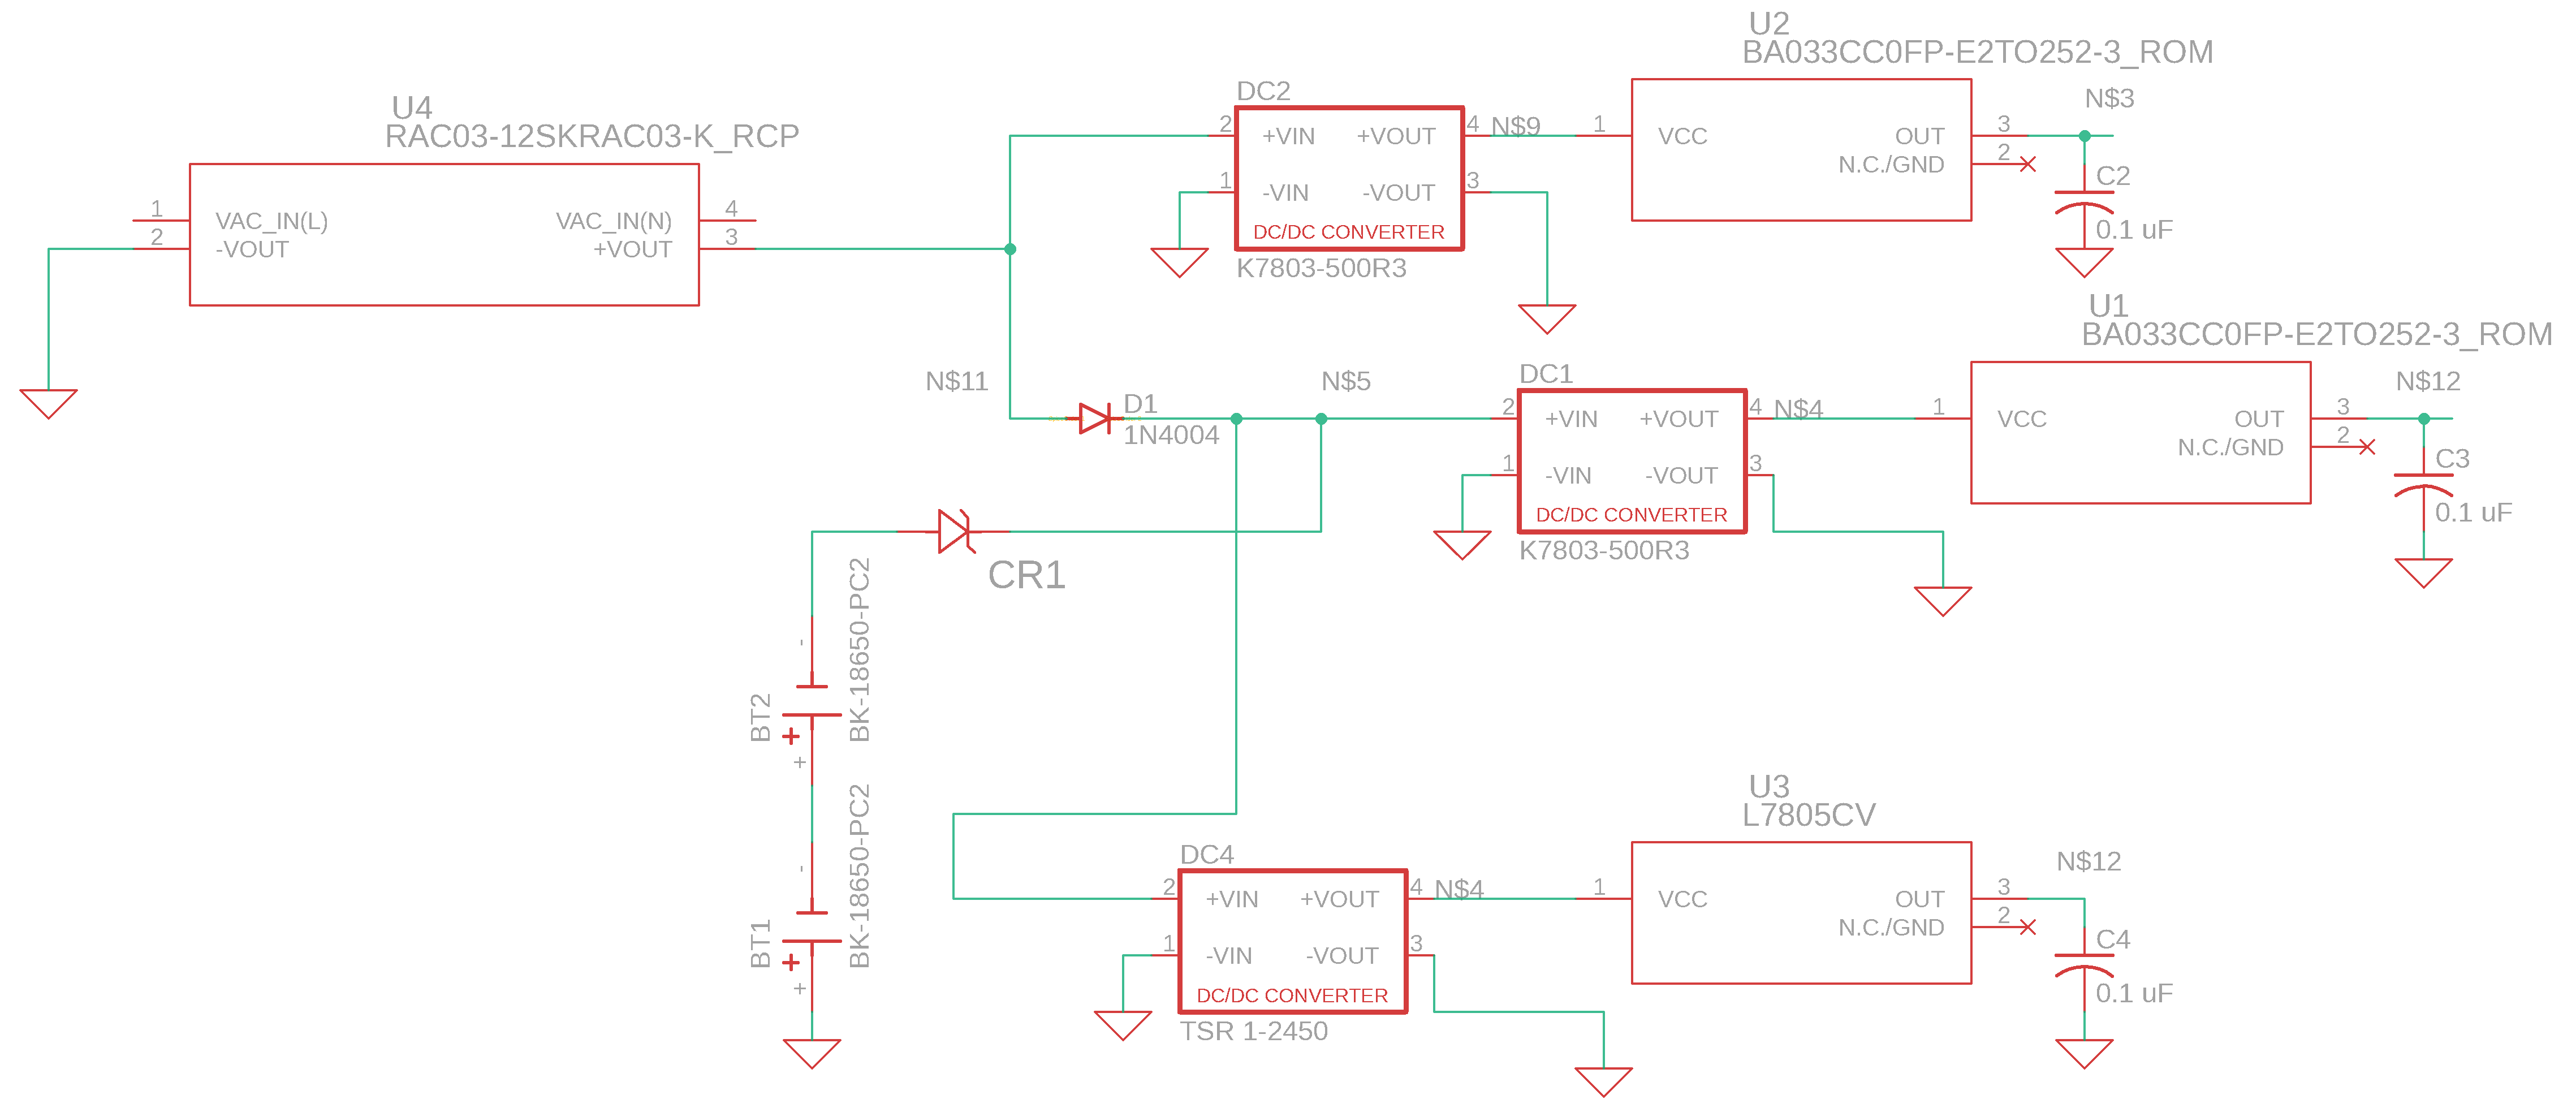
\includegraphics[width=1.6\textwidth, left]{../Modular Design/Main-Unit-PSU/Figures/main-unit-psu.png}
    \caption{Main Unit PSU Schematic}
    \label{fig:main-psu-schematic}
  \end{figure}
  \end{center}
\end{landscape}
\subsubsection{Power Analysis, Loading, Driving, and Compatibility}
According to the RAC03-12SK data sheet\cite{RAC0312SK}, the AC/DC converter can handle from 85\si{\V}AC to 264\si{\V}AC and produce 12\si{\V}DC at its output. Since this design will be tested in a 120\si{\V}AC electrical system, it is compatible.\\ At the output of the AC/DC converter, a 1N4004-G diode\cite{1N4004G} and a R78-E3.3-0.5 3.3\si{\V} DC/DC converter\cite{R78E330} (DC2) are placed in parallel. For DC2, according to its data sheet, is compatible within a voltage range of 6\si{\V} to 28\si{\V}. Since DC2 is at the output of the 12\si{\V} AC/DC converter, it is compatible.\\ At the node at the right of D1 (N\$5), when mains power is available is calculated as follows:
\begin{equation}
  V_{N\$5} = 12 -  V_{D}
  \label{eq:mains-batt-node-eqation-mains-available}
\end{equation}
where $V_{D}$ is the diode drop of the 1N4004-G which according to its data sheet is 1.1\si{\V}, resulting in $N\$5$ equal to 10.9\si{\V}. When there is mains power available, the node will be at 10.9\si{\V}, the batteries will be trying to conduct but since the voltage of the two 3.6\si{\V} cells in series will be 7.2\si{\V}, minus the diode drop of CR1\cite{1N5819} will be $7.2 - 0.55 = 6.65\si{\V}$. Therefore, the potential difference between mains power and battery power is $-4.25\si{\V}$, therefore CR1 will be placed in reverse bias and thus the batteries will not conduct, but since the negative potential difference is low, it is compatible, according to the 1N5819 data sheet\cite{1N5819}.\\ When mains power is available DC1, another K7803-500R3, will receive a voltage of 10.9\si{\V} and as mentioned above is compatible and will produce a 3.3\si{\V} output. At the outputs of both DC1,DC2 there are identical 3.3\si{\V} LDOs (BA33BC0T)\cite{BA33BC0T}, which according to their data sheet can accept up to 16\si{\V} which is compatible since U1 and U2 are being supplied by 3.3\si{\V} DC/DC converters and thus are compatible. At the outputs of U1 and U2 are C2 and C3 respectively, that are 0.1\si{\micro\farad} filtering capacitors whose voltage rating is 50\si{\V} which are compatible.\\ Going back to $N\$5$ DC4 (5\si{\V} DC/DC converter) is in parallel with DC1, thus when there is mains power available, will be supplied 10.9\si{\V}. According to the TSR 1-2450 (DC4) data sheet\cite{TSR12450} it can accept a DC voltage from 6.5\si{\V} to 36\si{\V} thus making it compatible and will output 5\si{\V} DC. At the output of DC4, a 5\si{\V} LDO is fed (L7805CV
), whose data sheet\cite{L7805CV} says that it can handle up to 36\si{\V} thus making it compatible since the output of DC4 is 5\si{\V}. Similarly to C3 and C4, a 0.1\si{\micro\farad} capacitor is placed in parallel with the output and is compatible since it has the same voltage rating of 50\si{\V}.\\ When mains power is not available DC2 will shutdown and D1 will be placed in reverse bias since CR1 will be conducting due to $N\$5$ will be at 0\si{\V} when mains power is not available and then will be placed at 6.65\si{\V}. Since DC1, DC2 and DC4 all have a minimum voltage less than 6.65\si{\V} they are all compatible and the LDOs and capacitors will operate as normal.
\subsubsection{Reliability \& Design Criteria}
The power supply for the main unit has to be working 100\% of the time since the main unit is required for the operation of the system. Because of this requirement the main power supply has an integrated battery backup switches automatically when mains power is not available and then can last for an extended period of time without the mains power available.
\subsubsection{Level of Completion}
\begin{table}[!ht]
  \begin{tabularx}{\textwidth}{|X|X|}
    \hline
    \multicolumn{2}{|X|}{Main Unit PSU}\\
    \hline
    Integration&\begin{itemize}
                  \item 4\si{\V} Power Rail
                  \item 3.3\si{\V} Power Rail
                  \item 3.3\si{\V} Power Sense
                  \item Automatic Power Source Switching
                \end{itemize}\\
    \hline
  \end{tabularx}
\end{table}
